
\section{Généralités}

Avant de commencer un projet de ce type, il est très important de se renseigner sur ce qu'attendent les futurs utilisateurs de notre application, afin de pouvoir guider notre conception et ainsi ne pas développer des fonctionnalités qui ne trouveraient pas leur public. De plus, nous ne souhaitons pas restreindre l'application au campus, et de ce fait le recueil des besoin doit aussi se faire sur d'autres campus, qui n'auraient pas la même disposition et donc auraient d'autres besoins. C’est dans cette optique que nous avons décidé de concevoir un questionnaire que nous pourrions envoyer au plus grand nombre, et ce dans toute la France.

\section{Conception du questionnaire}

Le questionnaire que nous avons conçu s'oriente vers deux axes principaux : identifier les informations qui pourraient intéresser les utilisateurs et les fonctionnalités qui pourraient leur plaire. \newline
Pour ce faire, nous avons préalablement déterminé un ensemble d'informations qui nous semblent pertinentes pour différents points de l'application. Par exemple, quels points de restauration prendre en compte, quels indicateurs afficher pour permettre aux utilisateurs de faire un choix parmi ces derniers. Pour ces questions, nous avons conçu des questions à choix restreints, c'est-à-dire que nous ne demandons pas simplement une réponse oui/non, mais une réponse qui apporte plus de nuance, comme une quantification de la fréquentation, ou des questions à choix multiples. Cela nous permet d'avoir des résultats pour lesquels on peut prendre en compte l'avis des utilisateurs qui ont des habitudes minoritaires par rapport aux autres. \newline
Quant aux propositions de fonctionnalités, nous avons choisi de proposer des idées et de les soumettre à l'avis des utilisateurs grâce à des réponses fermées, c'est-à-dire que nous voulons juste recueillir un avis de type intéressé/pas intéressé. Les utilisateurs ont souvent du mal à exprimer ce qu'ils souhaitent avoir exactement dans les programmes que l’on essaye de développer pour eux. Ainsi, en exprimant une idée sous cette forme, donc en demandant simplement son approbation, il peut facilement dire si l'idée lui semble pertinente ou non. Un champ libre en fin de questionnaire lui permet de proposer de nouvelles idées ou d'exprimer tout commentaire qu'il aurait envie de nous transmettre. \\

Une fois les questions identifiées, il a fallu soigner la rédaction et la présentation du questionnaire. En effet, un questionnaire de ce type est souvent rebutant du fait que les étudiants en reçoivent souvent et régulièrement à propos de différents projets. Ce questionnaire s'adressant plus particulièrement à des étudiants, nous avons donc essayé de le rendre attractif et convivial afin que les utilisateurs aient envie de le remplir du début à la fin, et ce en peu de temps.
Nous avons donc rédigé les questions une première fois, puis l'avons fait essayer à quelques camarades. Nous nous sommes vite rendu compte que ces dernières manquaient d'homogénéité et n'invitaient pas forcément l'utilisateur à répondre. Par exemple, les questions portant sur les fonctionnalités étaient de la forme \og{}Si nous vous proposions de faire ceci, seriez-vous intéressé ? Super/Bof\fg{}. Les testeurs qui ont lu le questionnaire sous cette forme ont trouvé que cette formulation était trop classique et qu'ils ne se sentaient pas forcément impliqués. Nous avons donc repensé toutes les questions afin de les rendre plus directes et surtout homogènes entre elles, notamment en utilisant le tutoiement. Les questions sur les fonctionnalités ressemblent maintenant à \og{}Faire ceci, ça t'intéresse ? Intéressé/Pas intéressé\fg{}. \newline
Au niveau de la forme, nous n'avons pas voulu utiliser le classique Google Form, qui est déjà trop utilisé autour de nous. De plus, Google Form renvoie l'image d’un questionnaire long et formel, ce qui n'était pas du tout en accord avec l'esprit de notre formulaire. Pour rappel, notre questionnaire se veut direct, convivial et accessible. Nous nous sommes finalement tournés vers Typeform, qui propose de réaliser des sondages multi-plateformes (gérant déjà le responsive pour les smartphones et tablettes), pour lequel on peut incorporer des icônes dans les réponses, permettant une lisibilité et accessibilité accrue. Avec son design moderne et ses outils de personnalisation, nous avons réussi à créer le questionnaire que nous avions imaginé. \\

Quelques retours utilisateurs sur notre questionnaire final :\\
\begin{description}
    \item \og{}Pas mal le formulaire\fg{}
    \item \og{}Superbe formulaire !\fg{}
    \item \og{}Excellent questionnaire avec un bon humour\fg{}
    \item \og{}Niveau approche des étudiants c’est super\fg{}
\end{description}

\begin{figure}[H]
    \label{fig-qcm-question}
    \noindent\makebox[\textwidth]{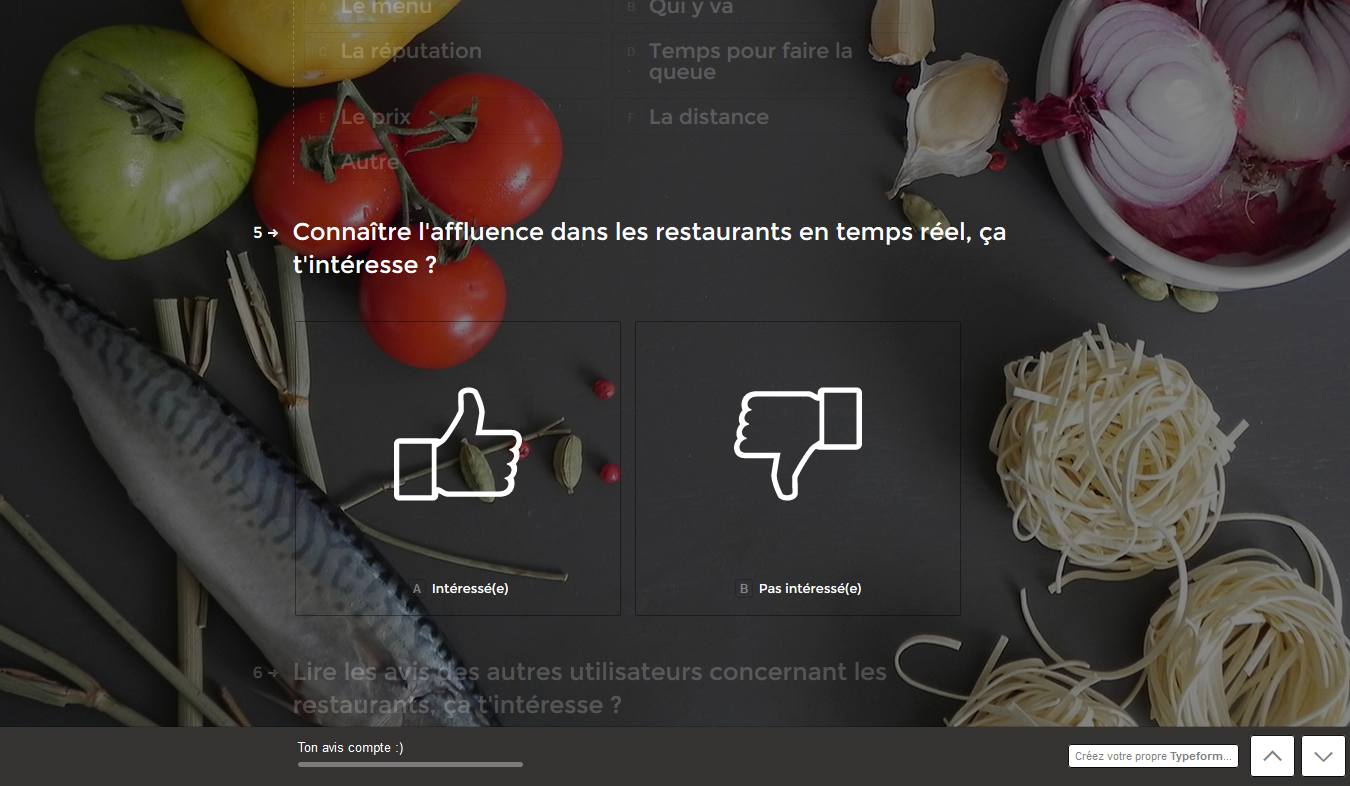
\includegraphics[width=10cm]{figures/qcm_question.png}}
    \caption{Capture d'écran d'une question du questionnaire}
\end{figure}

\section{Obtention et analyse des résultats}

Afin de réaliser une analyse multi-sites des besoins des potentiels utilisateurs de l'application, le questionnaire a été diffusé au sein de plusieurs campus de France, permettant ainsi d'obtenir des réponses de différentes régions. En effet, il est intéressant de combiner les besoins de différents profils d'utilisateurs, qui partagent tout de même une problématique commune. Ainsi, des réponses ont majoritairement été obtenues depuis les régions Auvergne, Bretagne, Centre et Rhône-Alpes. \\


\begin{figure}[H]
    \label{fig-carte-reponses}
    \noindent\makebox[\textwidth]{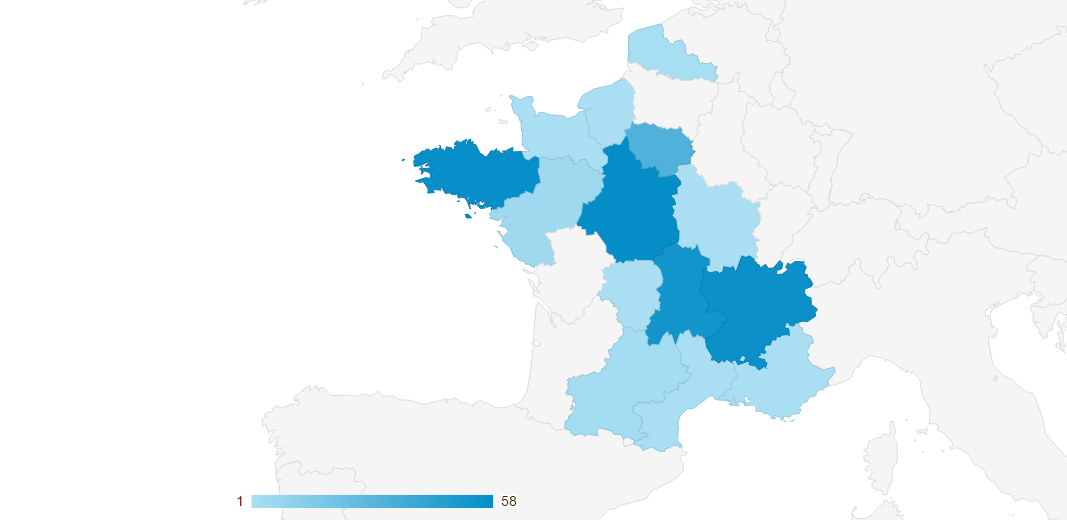
\includegraphics[width=10cm]{figures/carte_reponses.png}}
    \caption{Carte montrant la densité de réponses par régions}
\end{figure}

\begin{figure}[H]
    \label{fig-histo-reponses}
    \noindent\makebox[\textwidth]{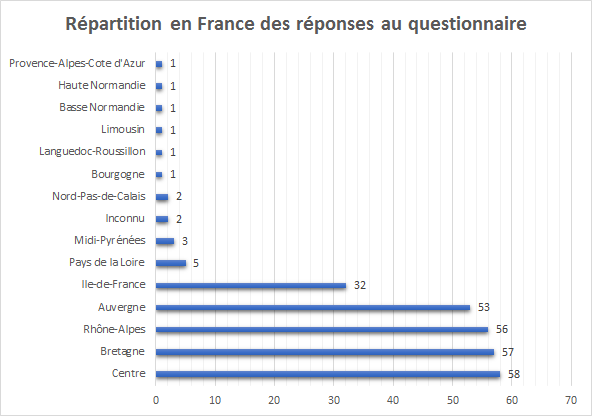
\includegraphics[width=10cm]{figures/histo_reponses.png}}
    \caption{Histogramme donnant le nombre de réponses par région}
\end{figure}

Grâce à cette diffusion inter-campus du questionnaire, 311 réponses ont été collectées. Certains internautes masquant leur position géographique lors de leur navigation, une légère différence est à relever entre le nombre de réponses total apparaissant sur le questionnaire et sur les graphiques de répartition géographique. L'ensemble des questions et des réponses associées sont disponibles en annexe A. \\

L'échantillon visé étant une population étudiante, 91\% des répondants ont déclaré posséder un smartphone, confortant ainsi l'idée de développer une application mobile. En effet, 80\% des répondants ont également déclaré être intéressés par une application smartphone permettant de connaître les différents points de restauration autour de leur campus. Ce pourcentage est suffisamment significatif pour s'intéresser dans un second temps aux habitudes et aux besoins des étudiants. \\

Ainsi, au cours d'une semaine type, 68\% des répondants mangent souvent voire tout le temps dans un restaurant universitaire. Cependant, 18\% des étudiants interrogés mangent très peu voir jamais dans un restaurant universitaire. En effet, 35\% des étudiants déjeunent parfois dans un restaurant/snack situé en dehors du campus, tandis que 20\% des étudiants mangent de temps en temps un repas acheté au supermarché. Cette hétérogénéité des réponses illustre bien les différentes habitudes des étudiants au sein des différents campus universitaires. Ainsi, il est important d'indiquer dans notre application non seulement les restaurants universitaires, mais également les différentes alternatives, afin de répondre aux besoins de chacun. \\

Afin de déterminer quelles sont les informations à mettre en avant dans notre application, nous pouvons nous intéresser aux différents critères identifiés comme importants par les étudiants ayant répondu au questionnaire. Ainsi, 82\% des répondants considèrent le prix comme étant un critère important lorsqu'ils recherchent un endroit pour manger. 66\% des étudiants considèrent également la distance et le temps d'attente comme étant importants, tandis que la réputation est un critère important pour seulement 12\% des répondants. De ce fait, notre application devra mettre en avant ces trois informations (prix, distance et temps d'attente) jugées comme critiques pour effectuer un choix. Ces données devront donc être visibles dès l'affichage réduit des lieux de restauration, les autres informations jugées comme étant moins importantes pouvant alors être visibles lors d’un affichage détaillé. \\

De même, 87\% des étudiants ayant répondu au questionnaire ont déclaré être intéressés pour connaître en temps réel l'affluence des lieux de restauration. Ce pourcentage fortement significatif concorde avec la déclaration de l'importance du critère du temps d'attente pour choisir un lieu de restauration. Cette donnée étant particulièrement importante, il est nécessaire d'indiquer des valeurs s'approchant au mieux de la situation réelle. Pour cela, une interface pour restaurateurs est à prévoir dans notre application, afin de permettre à ces derniers de renseigner à intervalles réguliers l’affluence de leur établissement. \\

Parmi les répondants au questionnaire, 77\% sont également intéressés par les avis des autres utilisateurs de l'application, sans pour autant rechercher un établissement présentant une haute réputation, cherchant ainsi les compromis. Nous pouvons donc prévoir un système d’évaluation des lieux de restauration par les utilisateurs de l'application, en demandant toutefois une notation numérique ainsi qu’une appréciation textuelle. Cela permettra de proposer dans un premier temps une notation moyenne. Dans un second temps, l'utilisateur aura la possibilité d'afficher l’ensemble des évaluations des utilisateurs, répondant ainsi au besoin exprimé à travers cette question. \\

A contrario, seulement 55\% des répondants sont intéressés par des informations diététiques sur les lieux de restauration et 45\% des étudiants ayant répondu sont intéressés par les avertissements et informations liés aux régimes particuliers. S'agissant de données importantes pour une minorité d'utilisateurs, ces informations pourront être paramétrées dans l'application afin d'activer leur affichage. \\

Concernant les fonctionnalités liées à la dimension sociale, celles-ci ne seront pas mises en avant dans l'application. En effet, 67\% des répondants présentent un intérêt pour la possibilité de convenir de rendez-vous avec leurs amis, tandis que seulement 32\% des étudiants souhaitent connaître les repas de leurs amis. Or, de nombreux outils existant permettant déjà de convenir d'un rendez-vous entre amis. Cette possibilité recueille en effet un bon pourcentage d'intérêt. Cependant, nombre de réactions négatives ont également été reçues quant à cette fonctionnalité. Ainsi, notre application ne comportera pas cette dimension sociale, afin de ne pas contraindre les utilisateurs sur le moyen de communication. \\

Le questionnaire comportait également un champ libre, permettant ainsi aux répondants de s'exprimer librement sur leurs besoins. Globalement, le concept de l’application a été bien accueilli, les étudiants émettant parfois leur souhait de voir l'application se réaliser afin de pouvoir l’utiliser par la suite. Ainsi, ce questionnaire nous a permis d'évaluer les différents besoins des étudiants à travers plusieurs campus qui présentent une même problématique, à savoir comment déterminer le lieu de restauration. Les informations à mettre en avant ont ainsi été déterminées, tandis que le bien fondé de l'application a été validé à travers ce questionnaire et son analyse. \\
